\documentclass[12pt,]{article}
\usepackage{lmodern}
\usepackage{amssymb,amsmath}
\usepackage{ifxetex,ifluatex}
\usepackage{fixltx2e} % provides \textsubscript
\ifnum 0\ifxetex 1\fi\ifluatex 1\fi=0 % if pdftex
  \usepackage[T1]{fontenc}
  \usepackage[utf8]{inputenc}
\else % if luatex or xelatex
  \ifxetex
    \usepackage{mathspec}
  \else
    \usepackage{fontspec}
  \fi
  \defaultfontfeatures{Ligatures=TeX,Scale=MatchLowercase}
    \setmainfont[]{Times New Roman}
\fi
% use upquote if available, for straight quotes in verbatim environments
\IfFileExists{upquote.sty}{\usepackage{upquote}}{}
% use microtype if available
\IfFileExists{microtype.sty}{%
\usepackage{microtype}
\UseMicrotypeSet[protrusion]{basicmath} % disable protrusion for tt fonts
}{}
\usepackage[margin=2.54cm]{geometry}
\usepackage{hyperref}
\hypersetup{unicode=true,
            pdftitle={Assessing water level changes from hurricanes from 2000 - 2020},
            pdfauthor={Camila Zarate Ospina, Savannah Artusi, and Autumn Dunn},
            pdfborder={0 0 0},
            breaklinks=true}
\urlstyle{same}  % don't use monospace font for urls
\usepackage{color}
\usepackage{fancyvrb}
\newcommand{\VerbBar}{|}
\newcommand{\VERB}{\Verb[commandchars=\\\{\}]}
\DefineVerbatimEnvironment{Highlighting}{Verbatim}{commandchars=\\\{\}}
% Add ',fontsize=\small' for more characters per line
\usepackage{framed}
\definecolor{shadecolor}{RGB}{248,248,248}
\newenvironment{Shaded}{\begin{snugshade}}{\end{snugshade}}
\newcommand{\AlertTok}[1]{\textcolor[rgb]{0.94,0.16,0.16}{#1}}
\newcommand{\AnnotationTok}[1]{\textcolor[rgb]{0.56,0.35,0.01}{\textbf{\textit{#1}}}}
\newcommand{\AttributeTok}[1]{\textcolor[rgb]{0.77,0.63,0.00}{#1}}
\newcommand{\BaseNTok}[1]{\textcolor[rgb]{0.00,0.00,0.81}{#1}}
\newcommand{\BuiltInTok}[1]{#1}
\newcommand{\CharTok}[1]{\textcolor[rgb]{0.31,0.60,0.02}{#1}}
\newcommand{\CommentTok}[1]{\textcolor[rgb]{0.56,0.35,0.01}{\textit{#1}}}
\newcommand{\CommentVarTok}[1]{\textcolor[rgb]{0.56,0.35,0.01}{\textbf{\textit{#1}}}}
\newcommand{\ConstantTok}[1]{\textcolor[rgb]{0.00,0.00,0.00}{#1}}
\newcommand{\ControlFlowTok}[1]{\textcolor[rgb]{0.13,0.29,0.53}{\textbf{#1}}}
\newcommand{\DataTypeTok}[1]{\textcolor[rgb]{0.13,0.29,0.53}{#1}}
\newcommand{\DecValTok}[1]{\textcolor[rgb]{0.00,0.00,0.81}{#1}}
\newcommand{\DocumentationTok}[1]{\textcolor[rgb]{0.56,0.35,0.01}{\textbf{\textit{#1}}}}
\newcommand{\ErrorTok}[1]{\textcolor[rgb]{0.64,0.00,0.00}{\textbf{#1}}}
\newcommand{\ExtensionTok}[1]{#1}
\newcommand{\FloatTok}[1]{\textcolor[rgb]{0.00,0.00,0.81}{#1}}
\newcommand{\FunctionTok}[1]{\textcolor[rgb]{0.00,0.00,0.00}{#1}}
\newcommand{\ImportTok}[1]{#1}
\newcommand{\InformationTok}[1]{\textcolor[rgb]{0.56,0.35,0.01}{\textbf{\textit{#1}}}}
\newcommand{\KeywordTok}[1]{\textcolor[rgb]{0.13,0.29,0.53}{\textbf{#1}}}
\newcommand{\NormalTok}[1]{#1}
\newcommand{\OperatorTok}[1]{\textcolor[rgb]{0.81,0.36,0.00}{\textbf{#1}}}
\newcommand{\OtherTok}[1]{\textcolor[rgb]{0.56,0.35,0.01}{#1}}
\newcommand{\PreprocessorTok}[1]{\textcolor[rgb]{0.56,0.35,0.01}{\textit{#1}}}
\newcommand{\RegionMarkerTok}[1]{#1}
\newcommand{\SpecialCharTok}[1]{\textcolor[rgb]{0.00,0.00,0.00}{#1}}
\newcommand{\SpecialStringTok}[1]{\textcolor[rgb]{0.31,0.60,0.02}{#1}}
\newcommand{\StringTok}[1]{\textcolor[rgb]{0.31,0.60,0.02}{#1}}
\newcommand{\VariableTok}[1]{\textcolor[rgb]{0.00,0.00,0.00}{#1}}
\newcommand{\VerbatimStringTok}[1]{\textcolor[rgb]{0.31,0.60,0.02}{#1}}
\newcommand{\WarningTok}[1]{\textcolor[rgb]{0.56,0.35,0.01}{\textbf{\textit{#1}}}}
\usepackage{graphicx,grffile}
\makeatletter
\def\maxwidth{\ifdim\Gin@nat@width>\linewidth\linewidth\else\Gin@nat@width\fi}
\def\maxheight{\ifdim\Gin@nat@height>\textheight\textheight\else\Gin@nat@height\fi}
\makeatother
% Scale images if necessary, so that they will not overflow the page
% margins by default, and it is still possible to overwrite the defaults
% using explicit options in \includegraphics[width, height, ...]{}
\setkeys{Gin}{width=\maxwidth,height=\maxheight,keepaspectratio}
\IfFileExists{parskip.sty}{%
\usepackage{parskip}
}{% else
\setlength{\parindent}{0pt}
\setlength{\parskip}{6pt plus 2pt minus 1pt}
}
\setlength{\emergencystretch}{3em}  % prevent overfull lines
\providecommand{\tightlist}{%
  \setlength{\itemsep}{0pt}\setlength{\parskip}{0pt}}
\setcounter{secnumdepth}{5}
% Redefines (sub)paragraphs to behave more like sections
\ifx\paragraph\undefined\else
\let\oldparagraph\paragraph
\renewcommand{\paragraph}[1]{\oldparagraph{#1}\mbox{}}
\fi
\ifx\subparagraph\undefined\else
\let\oldsubparagraph\subparagraph
\renewcommand{\subparagraph}[1]{\oldsubparagraph{#1}\mbox{}}
\fi

%%% Use protect on footnotes to avoid problems with footnotes in titles
\let\rmarkdownfootnote\footnote%
\def\footnote{\protect\rmarkdownfootnote}

%%% Change title format to be more compact
\usepackage{titling}

% Create subtitle command for use in maketitle
\providecommand{\subtitle}[1]{
  \posttitle{
    \begin{center}\large#1\end{center}
    }
}

\setlength{\droptitle}{-2em}

  \title{Assessing water level changes from hurricanes from 2000 - 2020}
    \pretitle{\vspace{\droptitle}\centering\huge}
  \posttitle{\par}
  \subtitle{\url{https://github.com/Autumn41/Dunn-Artusi-Zarate_ENV872_Project.git}}
  \author{Camila Zarate Ospina, Savannah Artusi, and Autumn Dunn}
    \preauthor{\centering\large\emph}
  \postauthor{\par}
    \date{}
    \predate{}\postdate{}
  
\usepackage{booktabs}
\usepackage{longtable}
\usepackage{array}
\usepackage{multirow}
\usepackage{wrapfig}
\usepackage{float}
\usepackage{colortbl}
\usepackage{pdflscape}
\usepackage{tabu}
\usepackage{threeparttable}
\usepackage{threeparttablex}
\usepackage[normalem]{ulem}
\usepackage{makecell}
\usepackage{xcolor}

\begin{document}
\maketitle

\newpage
\tableofcontents 
\newpage
\listoftables 
\newpage
\listoffigures 
\newpage

Set-Up Work Space

Input Raw Data

\begin{Shaded}
\begin{Highlighting}[]
\CommentTok{# Select Site}
\NormalTok{siteNo1 <-}\StringTok{"02137727"}
\NormalTok{siteNo2 <-}\StringTok{"02111000"}
\NormalTok{siteNo3 <-}\StringTok{"03446000"}
\NormalTok{siteNo4 <-}\StringTok{"03447687"}

\CommentTok{# Identify parameter of interest: }
\NormalTok{pcode =}\StringTok{ '00065'} \CommentTok{#gage height (feet)}

\CommentTok{# Identify statistic code for daily values: }
\NormalTok{scode =}\StringTok{ "00003"}  \CommentTok{#mean}

\CommentTok{# Identify start and end dates}
\NormalTok{start.date =}\StringTok{ "2000-01-01"}
\NormalTok{end.date =}\StringTok{ "2020-12-01"}

\CommentTok{# Load in data using the package's "readNWISdv" function}
\NormalTok{Catawba <-}\StringTok{ }\KeywordTok{readNWISdv}\NormalTok{(}\DataTypeTok{siteNumbers =}\NormalTok{ siteNo1, }
                    \DataTypeTok{parameterCd =}\NormalTok{ pcode, }
                    \DataTypeTok{statCd =}\NormalTok{ scode, }
                    \DataTypeTok{startDate=}\NormalTok{start.date, }
                    \DataTypeTok{endDate=}\NormalTok{end.date)}

\NormalTok{Yadkin <-}\StringTok{ }\KeywordTok{readNWISdv}\NormalTok{(}\DataTypeTok{siteNumbers =}\NormalTok{ siteNo2, }
                    \DataTypeTok{parameterCd =}\NormalTok{ pcode, }
                    \DataTypeTok{statCd =}\NormalTok{ scode, }
                    \DataTypeTok{startDate=}\NormalTok{start.date, }
                    \DataTypeTok{endDate=}\NormalTok{end.date)}

\NormalTok{Mills <-}\StringTok{ }\KeywordTok{readNWISdv}\NormalTok{(}\DataTypeTok{siteNumbers =}\NormalTok{ siteNo3, }
                    \DataTypeTok{parameterCd =}\NormalTok{ pcode, }
                    \DataTypeTok{statCd =}\NormalTok{ scode, }
                    \DataTypeTok{startDate=}\NormalTok{start.date, }
                    \DataTypeTok{endDate=}\NormalTok{end.date)}

\NormalTok{FrenchBroad <-}\StringTok{ }\KeywordTok{readNWISdv}\NormalTok{(}\DataTypeTok{siteNumbers =}\NormalTok{ siteNo4, }
                    \DataTypeTok{parameterCd =}\NormalTok{ pcode, }
                    \DataTypeTok{statCd =}\NormalTok{ scode, }
                    \DataTypeTok{startDate=}\NormalTok{start.date, }
                    \DataTypeTok{endDate=}\NormalTok{end.date)}

\CommentTok{# Rename columns}
\NormalTok{Catawba <-}\StringTok{ }\KeywordTok{renameNWISColumns}\NormalTok{(Catawba); }
\KeywordTok{colnames}\NormalTok{(Catawba)}
\end{Highlighting}
\end{Shaded}

\begin{verbatim}
## [1] "agency_cd" "site_no"   "Date"      "GH"        "GH_cd"
\end{verbatim}

\begin{Shaded}
\begin{Highlighting}[]
\KeywordTok{saveRDS}\NormalTok{(Catawba, }\DataTypeTok{file =}\StringTok{"../Data/Raw/Catawba.rds"}\NormalTok{)}

\NormalTok{Yadkin <-}\StringTok{ }\KeywordTok{renameNWISColumns}\NormalTok{(Yadkin); }
\KeywordTok{colnames}\NormalTok{(Yadkin)}
\end{Highlighting}
\end{Shaded}

\begin{verbatim}
## [1] "agency_cd" "site_no"   "Date"      "GH"        "GH_cd"
\end{verbatim}

\begin{Shaded}
\begin{Highlighting}[]
\KeywordTok{saveRDS}\NormalTok{(Yadkin, }\DataTypeTok{file =}\StringTok{"../Data/Raw/Yadkin.rds"}\NormalTok{)}

\NormalTok{Mills <-}\StringTok{ }\KeywordTok{renameNWISColumns}\NormalTok{(Mills); }
\KeywordTok{colnames}\NormalTok{(Mills)}
\end{Highlighting}
\end{Shaded}

\begin{verbatim}
## [1] "agency_cd" "site_no"   "Date"      "GH"        "GH_cd"
\end{verbatim}

\begin{Shaded}
\begin{Highlighting}[]
\KeywordTok{saveRDS}\NormalTok{(Mills, }\DataTypeTok{file =}\StringTok{"../Data/Raw/Mills.rds"}\NormalTok{)}

\NormalTok{FrenchBroad <-}\StringTok{ }\KeywordTok{renameNWISColumns}\NormalTok{(FrenchBroad); }
\KeywordTok{saveRDS}\NormalTok{(FrenchBroad, }\DataTypeTok{file =}\StringTok{"../Data/Raw/FrenchBroad.rds"}\NormalTok{)}
\end{Highlighting}
\end{Shaded}

Process Data

\begin{Shaded}
\begin{Highlighting}[]
\CommentTok{#Catawba}
\NormalTok{Catawba}\OperatorTok{$}\NormalTok{Date<-}\KeywordTok{as.Date}\NormalTok{(Catawba}\OperatorTok{$}\NormalTok{Date, }\DataTypeTok{format =} \StringTok{"%Y/%m/%d"}\NormalTok{)}
\NormalTok{Catawba_sept <-}\StringTok{ }\NormalTok{Catawba }\OperatorTok\StringTok{ }
\StringTok{                  }\KeywordTok{select}\NormalTok{(Date, GH) }\OperatorTok\StringTok{ }
\StringTok{                  }\KeywordTok{mutate}\NormalTok{(}\DataTypeTok{Month =} \KeywordTok{month}\NormalTok{(Date),}
                         \DataTypeTok{Year =} \KeywordTok{year}\NormalTok{(Date)) }\OperatorTok\StringTok{ }
\StringTok{                  }\KeywordTok{filter}\NormalTok{(Month }\OperatorTok\StringTok{ }\NormalTok{(}\StringTok{"9"}\NormalTok{)) }\OperatorTok\StringTok{ }
\StringTok{                  }\KeywordTok{select}\NormalTok{(Date, GH, Year)}
\KeywordTok{saveRDS}\NormalTok{(Catawba_sept, }\DataTypeTok{file =}\StringTok{"../Data/Processed/Catawba_sept.rds"}\NormalTok{)}

\CommentTok{#Yadkin}
\NormalTok{Yadkin}\OperatorTok{$}\NormalTok{Date<-}\KeywordTok{as.Date}\NormalTok{(Yadkin}\OperatorTok{$}\NormalTok{Date, }\DataTypeTok{format =} \StringTok{"%Y/%m/%d"}\NormalTok{)}
\NormalTok{Yadkin_sept <-}\StringTok{ }\NormalTok{Yadkin }\OperatorTok\StringTok{ }
\StringTok{                  }\KeywordTok{select}\NormalTok{(Date, GH) }\OperatorTok\StringTok{ }
\StringTok{                  }\KeywordTok{mutate}\NormalTok{(}\DataTypeTok{Month =} \KeywordTok{month}\NormalTok{(Date),}
                         \DataTypeTok{Year =} \KeywordTok{year}\NormalTok{(Date)) }\OperatorTok\StringTok{ }
\StringTok{                  }\KeywordTok{filter}\NormalTok{(Month }\OperatorTok\StringTok{ }\NormalTok{(}\StringTok{"9"}\NormalTok{)) }\OperatorTok\StringTok{ }
\StringTok{                  }\KeywordTok{select}\NormalTok{(Date, GH, Year)}
\KeywordTok{saveRDS}\NormalTok{(Yadkin_sept, }\DataTypeTok{file =}\StringTok{"../Data/Processed/Yadkin_sept.rds"}\NormalTok{)}

\CommentTok{#Mills}
\NormalTok{Mills}\OperatorTok{$}\NormalTok{Date<-}\KeywordTok{as.Date}\NormalTok{(Mills}\OperatorTok{$}\NormalTok{Date, }\DataTypeTok{format =} \StringTok{"%Y/%m/%d"}\NormalTok{)}
\NormalTok{Mills_sept <-}\StringTok{ }\NormalTok{Mills }\OperatorTok\StringTok{ }
\StringTok{                  }\KeywordTok{select}\NormalTok{(Date, GH) }\OperatorTok\StringTok{ }
\StringTok{                  }\KeywordTok{mutate}\NormalTok{(}\DataTypeTok{Month =} \KeywordTok{month}\NormalTok{(Date),}
                         \DataTypeTok{Year =} \KeywordTok{year}\NormalTok{(Date)) }\OperatorTok\StringTok{ }
\StringTok{                  }\KeywordTok{filter}\NormalTok{(Month }\OperatorTok\StringTok{ }\NormalTok{(}\StringTok{"9"}\NormalTok{)) }\OperatorTok\StringTok{ }
\StringTok{                  }\KeywordTok{select}\NormalTok{(Date, GH, Year)}
\KeywordTok{saveRDS}\NormalTok{(Mills_sept, }\DataTypeTok{file =}\StringTok{"../Data/Processed/Mills_sept.rds"}\NormalTok{)}

\CommentTok{#FrenchBroad}
\NormalTok{FrenchBroad}\OperatorTok{$}\NormalTok{Date<-}\KeywordTok{as.Date}\NormalTok{(FrenchBroad}\OperatorTok{$}\NormalTok{Date, }\DataTypeTok{format =} \StringTok{"%Y/%m/%d"}\NormalTok{)}
\NormalTok{FrenchBroad_sept <-}\StringTok{ }\NormalTok{FrenchBroad }\OperatorTok\StringTok{ }
\StringTok{                  }\KeywordTok{select}\NormalTok{(Date, GH) }\OperatorTok\StringTok{ }
\StringTok{                  }\KeywordTok{mutate}\NormalTok{(}\DataTypeTok{Month =} \KeywordTok{month}\NormalTok{(Date),}
                         \DataTypeTok{Year =} \KeywordTok{year}\NormalTok{(Date)) }\OperatorTok\StringTok{ }
\StringTok{                  }\KeywordTok{filter}\NormalTok{(Month }\OperatorTok\StringTok{ }\NormalTok{(}\StringTok{"9"}\NormalTok{)) }\OperatorTok\StringTok{ }
\StringTok{                  }\KeywordTok{select}\NormalTok{(Date, GH, Year)}
\KeywordTok{saveRDS}\NormalTok{(FrenchBroad_sept, }\DataTypeTok{file =}\StringTok{"../Data/Processed/FrenchBroad_sept.rds"}\NormalTok{)}
\end{Highlighting}
\end{Shaded}

\hypertarget{rationale-and-research-questions}{%
\section{Rationale and Research
Questions}\label{rationale-and-research-questions}}

From 2000 to 2020, North Carolina was hit with 64 hurricanes and 26 of
those hurricanes occurred in September. With climate change, hurricanes
are expected to occur more frequently and at higher intensity (Elsner,
2006). Higher intensity storms will likely cause flooding of cities and
urban areas which many infrastructures are not designed to accommodate
(James et al., 2020; Marsooli \& Lin, 2020). Additionally, much of North
Carolina Piedmont wetlands have been drained and many streams are
degraded due to urban disturbances(Carle, 2011; Violin et al., 2011).
Wetlands and streams are natural systems that store flood water, and
without them, many areas that have not flooded in the past will be at
risk (Ameli \& Creed, 2019). Investing in pre-disaster hazard mitigation
has been shown to be economically beneficial and save lives (Villa,
2020). In order to update infrastructure, expected water input and time
period of elevated water levels are needed. Using stream gage height, we
selected Catawba River, Yadkin River, Mills River, and French Broad
River, because of their location along the path of Hurrican Florence,
which hit North Carolina in 2018. We focused on two questions: has gage
height changed over 2000-2020 for September from hurricanes and how much
does a stream gage height change after a hurricane?

From 2000 to 2020, North Carolina was hit with 64 hurricanes and 26 of
those hurricanes occurred in September. With climate change, hurricanes
are expected to occur more frequently and at higher intensity (Elsner,
2006). Higher intensity storms will likely cause flooding of cities and
urban areas which many infrastructures are not designed to accommodate
(James et al., 2020; Marsooli \& Lin, 2020). Additionally, much of North
Carolina Piedmont wetlands have been drained and many streams are
degraded due to urban disturbances (Carle, 2011; Violin et al., 2011).
Wetlands and streams are natural systems that store flood water, and
without them, many areas that have not flooded in the past will be at
risk (Ameli \& Creed, 2019). Investing in pre-disaster hazard mitigation
has been shown to be economically beneficial and save lives (Villa,
2020). In order to update infrastructure, expected water input and time
period of elevated water levels are needed. Using stream gage height, we
selected Catawba River, Yadkin River, Mills River, and French Broad
River, because of their location along hurricane paths. We focused on
two questions: has gage height changed over 2000-2020 for September from
hurricanes and how much does a stream gage height change after a
hurricane?

\newpage

\hypertarget{dataset-information}{%
\section{Dataset Information}\label{dataset-information}}

Data were retrieved from USGS National Water Information. USGS uses an
eight digit code for each site (listed below). The parameter of
interest, represented as GH in the tables, was gage height (feet),
identified using the pcode 00065. Daily mean value was used, using the
scode 00003.

Site locations and site codes: River Names \textbar{} NC City \textbar{}
Site Code \textbar{}\\
-------------------\textbar{}------------------\textbar{}-----------\textbar{}
Catawba River \textbar{} Pleasant Gardens \textbar{} 02137727 \textbar{}
Yadkin River \textbar{} Patterson \textbar{} 02111000 \textbar{} Mills
River \textbar{} Mills River \textbar{} 03446000 \textbar{} French Broad
River \textbar{} (Fletcher) \textbar{} 03447687 \textbar{}

To process the data, gage heights for September for all available years
were selected from the raw gage height data. This was done by converting
the raw date to a recognized date format and filtering by month. Later,
to run the t-tests, each river dataset was subsetted into two datasets,
one for 2001 and one for 2018 for each river.

\newpage

\hypertarget{exploratory-analysis}{%
\section{Exploratory Analysis}\label{exploratory-analysis}}

\begin{Shaded}
\begin{Highlighting}[]
\CommentTok{#Plot 1 - Catawba Gage Height as points on individual plots for September}
\KeywordTok{ggplot}\NormalTok{(Catawba_sept, }\KeywordTok{aes}\NormalTok{(}\DataTypeTok{y=}\NormalTok{GH, }\DataTypeTok{x=}\NormalTok{Date)) }\OperatorTok{+}
\StringTok{  }\KeywordTok{geom_point}\NormalTok{() }\OperatorTok{+}
\StringTok{  }\KeywordTok{xlab}\NormalTok{(}\StringTok{"Date"}\NormalTok{) }\OperatorTok{+}
\StringTok{  }\KeywordTok{ylab}\NormalTok{(}\StringTok{"Gage Height (feet)"}\NormalTok{) }\OperatorTok{+}
\StringTok{  }\NormalTok{mytheme }\OperatorTok{+}
\StringTok{  }\KeywordTok{facet_wrap}\NormalTok{(}\KeywordTok{vars}\NormalTok{(Year)) }
\end{Highlighting}
\end{Shaded}

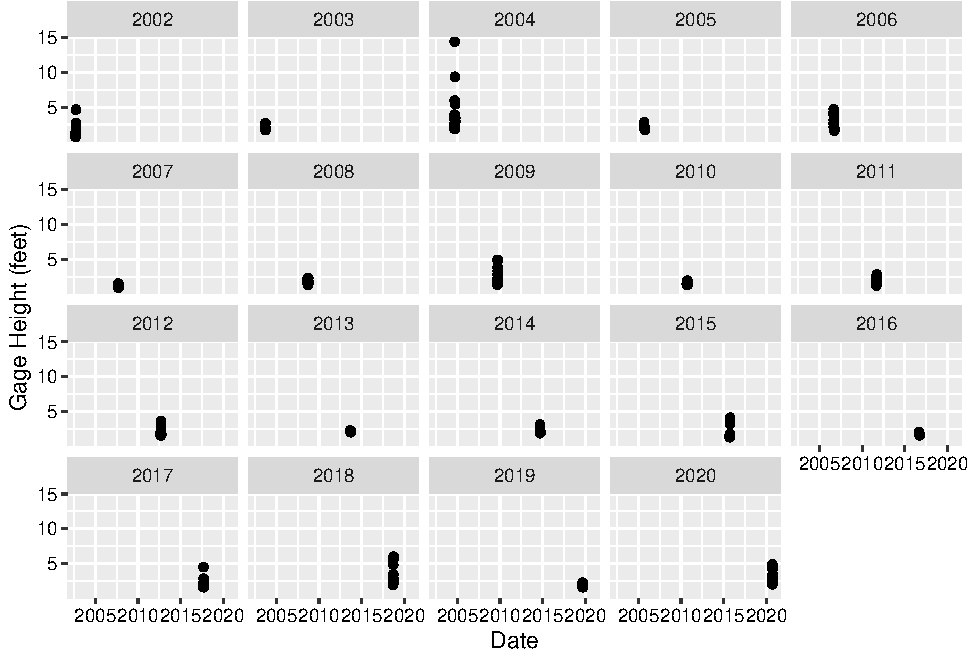
\includegraphics{Project_Template_files/figure-latex/Plots-1.pdf}

\begin{Shaded}
\begin{Highlighting}[]
\CommentTok{#Plot 2 - Yadkin Gage Height as points on individual plots for September}
\KeywordTok{ggplot}\NormalTok{(Yadkin_sept, }\KeywordTok{aes}\NormalTok{(}\DataTypeTok{y=}\NormalTok{GH, }\DataTypeTok{x=}\NormalTok{Date)) }\OperatorTok{+}
\StringTok{  }\KeywordTok{geom_point}\NormalTok{() }\OperatorTok{+}
\StringTok{  }\KeywordTok{xlab}\NormalTok{(}\StringTok{"Date"}\NormalTok{) }\OperatorTok{+}
\StringTok{  }\KeywordTok{ylab}\NormalTok{(}\StringTok{"Gage Height (feet)"}\NormalTok{) }\OperatorTok{+}
\StringTok{  }\NormalTok{mytheme }\OperatorTok{+}
\StringTok{  }\KeywordTok{facet_wrap}\NormalTok{(}\KeywordTok{vars}\NormalTok{(Year)) }
\end{Highlighting}
\end{Shaded}

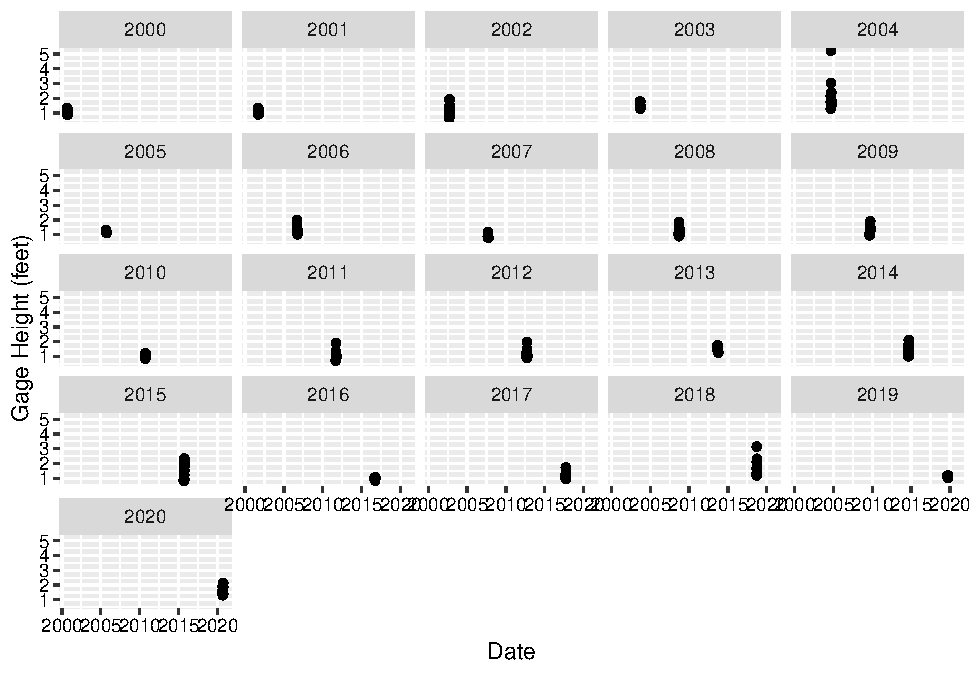
\includegraphics{Project_Template_files/figure-latex/Plots-2.pdf}

\begin{Shaded}
\begin{Highlighting}[]
\CommentTok{#Plot 3 - Mills Gage Height as points on individual plots for September}
\KeywordTok{ggplot}\NormalTok{(Mills_sept, }\KeywordTok{aes}\NormalTok{(}\DataTypeTok{y=}\NormalTok{GH, }\DataTypeTok{x=}\NormalTok{Date)) }\OperatorTok{+}
\StringTok{  }\KeywordTok{geom_point}\NormalTok{() }\OperatorTok{+}
\StringTok{  }\KeywordTok{xlab}\NormalTok{(}\StringTok{"Date"}\NormalTok{) }\OperatorTok{+}
\StringTok{  }\KeywordTok{ylab}\NormalTok{(}\StringTok{"Gage Height (feet)"}\NormalTok{) }\OperatorTok{+}
\StringTok{  }\NormalTok{mytheme }\OperatorTok{+}
\StringTok{  }\KeywordTok{facet_wrap}\NormalTok{(}\KeywordTok{vars}\NormalTok{(Year)) }
\end{Highlighting}
\end{Shaded}

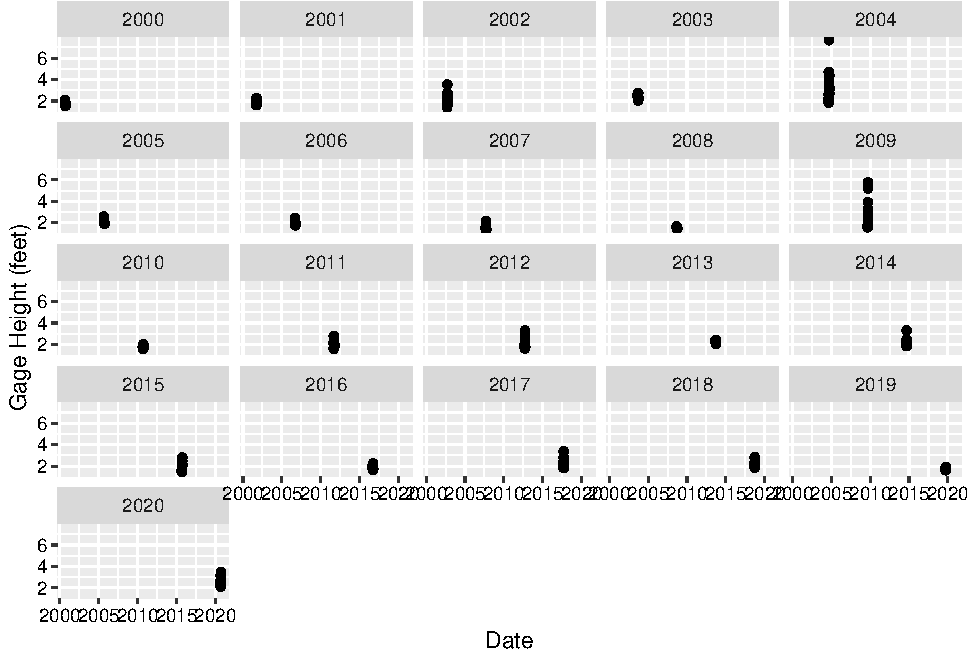
\includegraphics{Project_Template_files/figure-latex/Plots-3.pdf}

\begin{Shaded}
\begin{Highlighting}[]
\CommentTok{#Plot 4 - FrenchBroad Gage Height as points on individual plots for September}
\KeywordTok{ggplot}\NormalTok{(FrenchBroad_sept, }\KeywordTok{aes}\NormalTok{(}\DataTypeTok{y=}\NormalTok{GH, }\DataTypeTok{x=}\NormalTok{Date)) }\OperatorTok{+}
\StringTok{  }\KeywordTok{geom_point}\NormalTok{() }\OperatorTok{+}
\StringTok{  }\KeywordTok{xlab}\NormalTok{(}\StringTok{"Date"}\NormalTok{) }\OperatorTok{+}
\StringTok{  }\KeywordTok{ylab}\NormalTok{(}\StringTok{"Gage Height (feet)"}\NormalTok{) }\OperatorTok{+}
\StringTok{  }\NormalTok{mytheme }\OperatorTok{+}
\StringTok{  }\KeywordTok{facet_wrap}\NormalTok{(}\KeywordTok{vars}\NormalTok{(Year)) }
\end{Highlighting}
\end{Shaded}

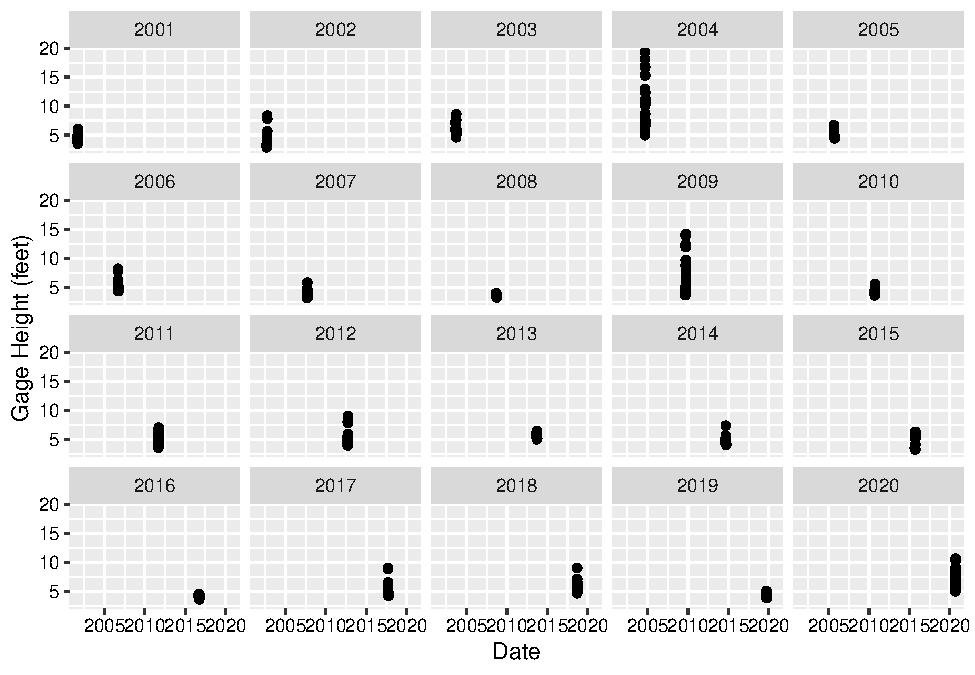
\includegraphics{Project_Template_files/figure-latex/Plots-4.pdf}

\newpage

\hypertarget{analysis}{%
\section{Analysis}\label{analysis}}

Time Series of four rivers from 2000 - 2020

\begin{Shaded}
\begin{Highlighting}[]
\CommentTok{## Catawba ##}

\CommentTok{# Generate time series}
\NormalTok{Start_month <-}\StringTok{ }\KeywordTok{month}\NormalTok{(}\KeywordTok{first}\NormalTok{(Catawba_sept))}
\NormalTok{Start_year <-}\StringTok{ }\KeywordTok{year}\NormalTok{(}\KeywordTok{first}\NormalTok{(Catawba_sept))}

\NormalTok{Catawba.daily.ts <-}\StringTok{ }\KeywordTok{ts}\NormalTok{(Catawba}\OperatorTok{$}\NormalTok{GH,}
                   \DataTypeTok{start=}\KeywordTok{c}\NormalTok{(Start_year,Start_month),}
                   \DataTypeTok{frequency=}\DecValTok{30}\NormalTok{) }

\CommentTok{# Decompose}
\NormalTok{Day_Catawba_decomp <-}\StringTok{ }\KeywordTok{stl}\NormalTok{(Catawba.daily.ts, }\DataTypeTok{s.window =} \StringTok{"periodic"}\NormalTok{)}
\KeywordTok{plot}\NormalTok{(Day_Catawba_decomp)}
\end{Highlighting}
\end{Shaded}

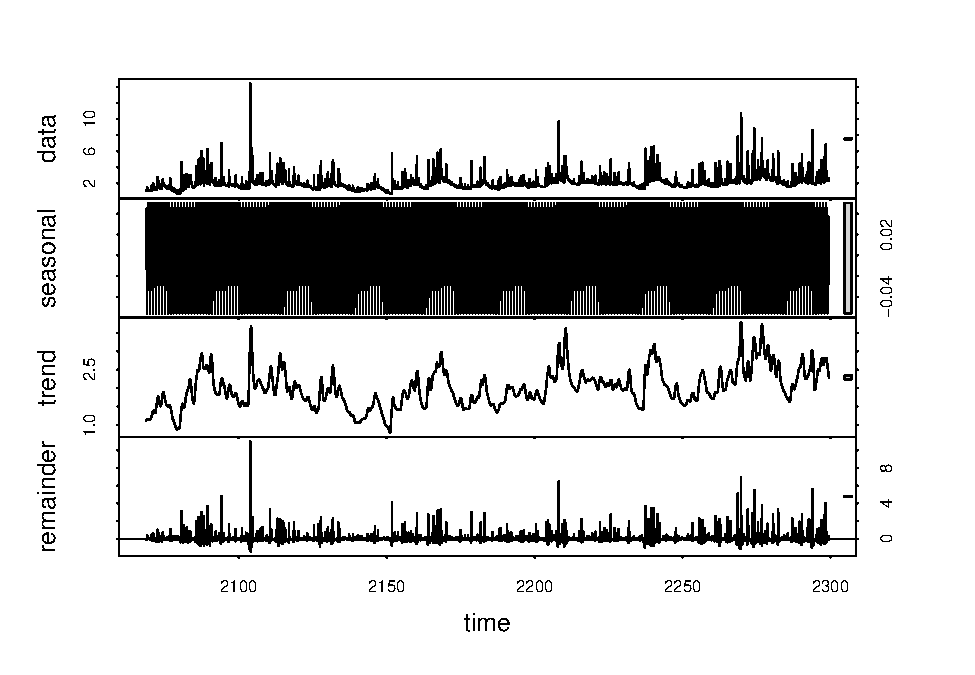
\includegraphics{Project_Template_files/figure-latex/TimeSeries-1.pdf}

\begin{Shaded}
\begin{Highlighting}[]
\CommentTok{# Run SMK test}
\NormalTok{Month_Catawba_trend <-}\StringTok{ }\NormalTok{Kendall}\OperatorTok{::}\KeywordTok{SeasonalMannKendall}\NormalTok{(Catawba.daily.ts)}

\CommentTok{# Inspect results}
\KeywordTok{summary}\NormalTok{(Month_Catawba_trend)}
\end{Highlighting}
\end{Shaded}

\begin{verbatim}
## Score =  208802 , Var(Score) = 41240024
## denominator =  793309.8
## tau = 0.263, 2-sided pvalue =< 2.22e-16
\end{verbatim}

\begin{Shaded}
\begin{Highlighting}[]
\CommentTok{## Yadkin ##}

\CommentTok{# Generate time series}
\NormalTok{Start_month2 <-}\StringTok{ }\KeywordTok{month}\NormalTok{(}\KeywordTok{first}\NormalTok{(Yadkin_sept))}
\NormalTok{Start_year2 <-}\StringTok{ }\KeywordTok{year}\NormalTok{(}\KeywordTok{first}\NormalTok{(Yadkin_sept))}

\NormalTok{Yadkin.daily.ts <-}\StringTok{ }\KeywordTok{ts}\NormalTok{(Yadkin}\OperatorTok{$}\NormalTok{GH,}
                   \DataTypeTok{start=}\KeywordTok{c}\NormalTok{(Start_year2,Start_month2),}
                   \DataTypeTok{frequency=}\DecValTok{30}\NormalTok{) }

\CommentTok{# Decompose}
\NormalTok{Day_Yadkin_decomp <-}\StringTok{ }\KeywordTok{stl}\NormalTok{(Yadkin.daily.ts, }\DataTypeTok{s.window =} \StringTok{"periodic"}\NormalTok{)}
\KeywordTok{plot}\NormalTok{(Day_Yadkin_decomp)}

\CommentTok{# Run SMK test}
\NormalTok{Month_Yadkin_trend <-}\StringTok{ }\NormalTok{Kendall}\OperatorTok{::}\KeywordTok{SeasonalMannKendall}\NormalTok{(Yadkin.daily.ts)}

\CommentTok{# Inspect results}
\KeywordTok{summary}\NormalTok{(Month_Yadkin_trend)}
\end{Highlighting}
\end{Shaded}

\begin{verbatim}
## Score =  130395 , Var(Score) = 54970729
## denominator =  959441.5
## tau = 0.136, 2-sided pvalue =< 2.22e-16
\end{verbatim}

\begin{Shaded}
\begin{Highlighting}[]
\CommentTok{## Mills ##}

\CommentTok{# Generate time series}
\NormalTok{Start_month3 <-}\StringTok{ }\KeywordTok{month}\NormalTok{(}\KeywordTok{first}\NormalTok{(Mills_sept))}
\NormalTok{Start_year3 <-}\StringTok{ }\KeywordTok{year}\NormalTok{(}\KeywordTok{first}\NormalTok{(Mills_sept))}

\NormalTok{Mills.daily.ts <-}\StringTok{ }\KeywordTok{ts}\NormalTok{(Yadkin}\OperatorTok{$}\NormalTok{GH,}
                   \DataTypeTok{start=}\KeywordTok{c}\NormalTok{(Start_year3,Start_month3),}
                   \DataTypeTok{frequency=}\DecValTok{30}\NormalTok{) }

\CommentTok{# Decompose}
\NormalTok{Day_Mills_decomp <-}\StringTok{ }\KeywordTok{stl}\NormalTok{(Mills.daily.ts, }\DataTypeTok{s.window =} \StringTok{"periodic"}\NormalTok{)}
\KeywordTok{plot}\NormalTok{(Day_Mills_decomp)}
\end{Highlighting}
\end{Shaded}

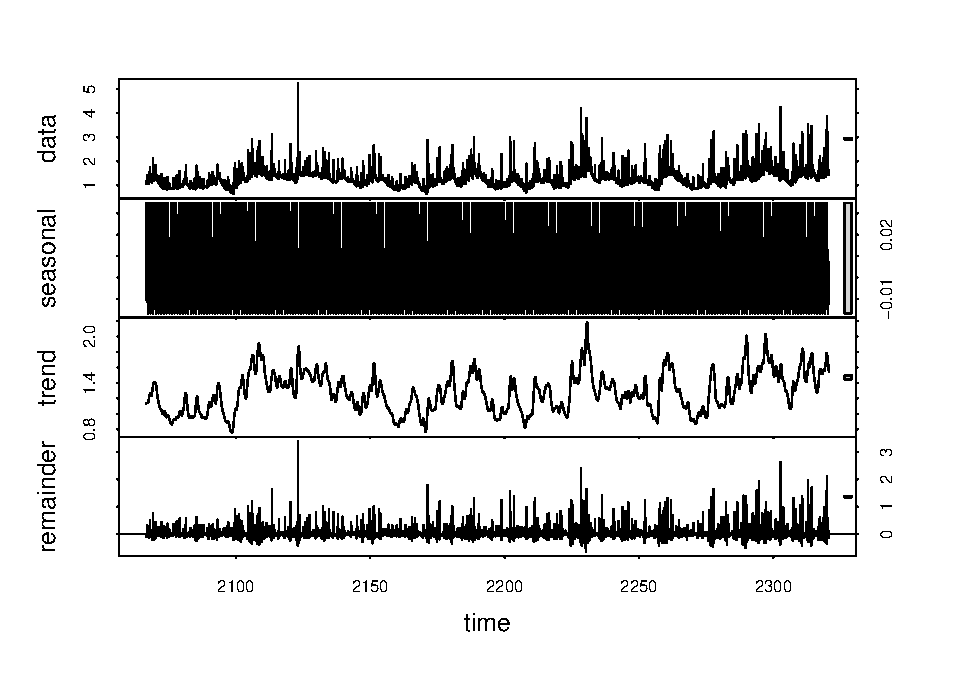
\includegraphics{Project_Template_files/figure-latex/TimeSeries-2.pdf}

\begin{Shaded}
\begin{Highlighting}[]
\CommentTok{# Run SMK test}
\NormalTok{Month_Mills_trend <-}\StringTok{ }\NormalTok{Kendall}\OperatorTok{::}\KeywordTok{SeasonalMannKendall}\NormalTok{(Mills.daily.ts)}

\CommentTok{# Inspect results}
\KeywordTok{summary}\NormalTok{(Month_Mills_trend)}
\end{Highlighting}
\end{Shaded}

\begin{verbatim}
## Score =  130395 , Var(Score) = 54970729
## denominator =  959441.5
## tau = 0.136, 2-sided pvalue =< 2.22e-16
\end{verbatim}

\begin{Shaded}
\begin{Highlighting}[]
\CommentTok{## FrenchBroad ##}

\CommentTok{# Generate time series}
\NormalTok{Start_month4 <-}\StringTok{ }\KeywordTok{month}\NormalTok{(}\KeywordTok{first}\NormalTok{(FrenchBroad_sept))}
\NormalTok{Start_year4<-}\StringTok{ }\KeywordTok{year}\NormalTok{(}\KeywordTok{first}\NormalTok{(FrenchBroad_sept))}

\NormalTok{FrenchBroad.daily.ts <-}\StringTok{ }\KeywordTok{ts}\NormalTok{(FrenchBroad}\OperatorTok{$}\NormalTok{GH,}
                   \DataTypeTok{start=}\KeywordTok{c}\NormalTok{(Start_year4,Start_month4),}
                   \DataTypeTok{frequency=}\DecValTok{30}\NormalTok{) }

\CommentTok{# Decompose}
\NormalTok{Day_FrenchBroad_decomp <-}\StringTok{ }\KeywordTok{stl}\NormalTok{(FrenchBroad.daily.ts, }\DataTypeTok{s.window =} \StringTok{"periodic"}\NormalTok{)}
\KeywordTok{plot}\NormalTok{(Day_FrenchBroad_decomp)}
\end{Highlighting}
\end{Shaded}

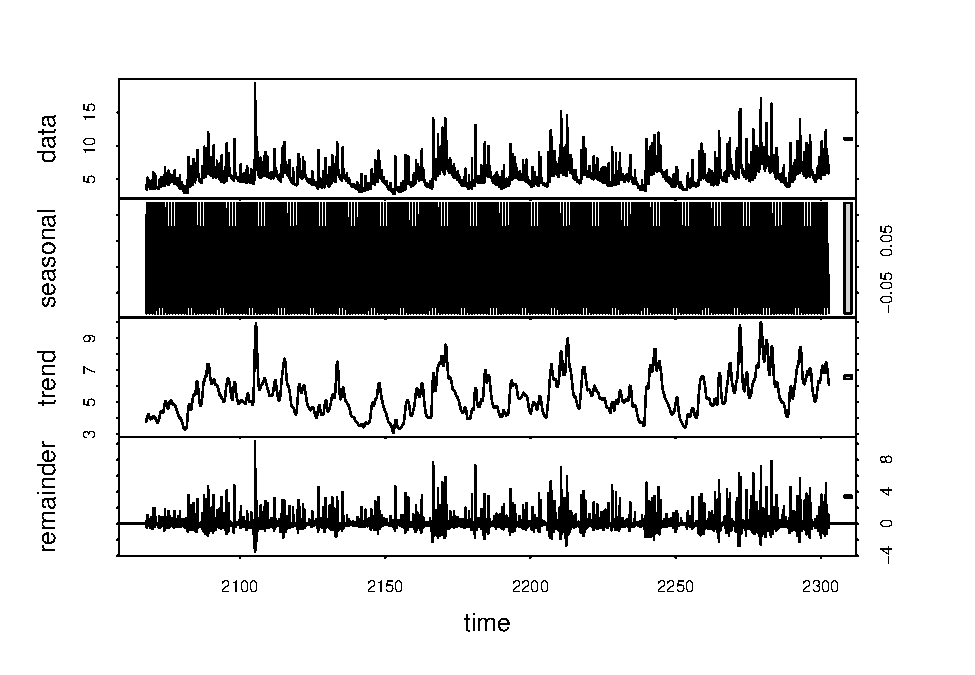
\includegraphics{Project_Template_files/figure-latex/TimeSeries-3.pdf}

\begin{Shaded}
\begin{Highlighting}[]
\CommentTok{# Run SMK test}
\NormalTok{Month_FrenchBroad_trend <-}\StringTok{ }\NormalTok{Kendall}\OperatorTok{::}\KeywordTok{SeasonalMannKendall}\NormalTok{(FrenchBroad.daily.ts)}

\CommentTok{# Inspect results}
\KeywordTok{summary}\NormalTok{(Month_FrenchBroad_trend)}
\end{Highlighting}
\end{Shaded}

\begin{verbatim}
## Score =  128036 , Var(Score) = 43605765
## denominator =  824809.4
## tau = 0.155, 2-sided pvalue =< 2.22e-16
\end{verbatim}

T-Test comparing September 2001 to 2018

\begin{Shaded}
\begin{Highlighting}[]
\CommentTok{#H0: Gage Height is the same in September for both years}
\CommentTok{#Ha: Gage Height is not the same in September for both years}

\CommentTok{## Yadkin - T-Test}
\CommentTok{# Create Dataframes}
\NormalTok{Yadkin_}\DecValTok{2001}\NormalTok{ <-}\StringTok{ }\NormalTok{Yadkin_sept }\OperatorTok\StringTok{ }\KeywordTok{filter}\NormalTok{(Year}\OperatorTok{==}\StringTok{ }\DecValTok{2001}\NormalTok{)}
\NormalTok{Yadkin_}\DecValTok{2018}\NormalTok{ <-}\StringTok{ }\NormalTok{Yadkin_sept }\OperatorTok\StringTok{ }\KeywordTok{filter}\NormalTok{(Year}\OperatorTok{==}\StringTok{ }\DecValTok{2018}\NormalTok{)}

\CommentTok{#Check assumptions}
\NormalTok{Yadkin_var <-}\StringTok{ }\KeywordTok{var.test}\NormalTok{(Yadkin_}\DecValTok{2001}\OperatorTok{$}\NormalTok{GH, Yadkin_}\DecValTok{2018}\OperatorTok{$}\NormalTok{GH)}
\KeywordTok{sd}\NormalTok{(Yadkin_}\DecValTok{2001}\OperatorTok{$}\NormalTok{GH)}\OperatorTok{/}\KeywordTok{sd}\NormalTok{(Yadkin_}\DecValTok{2018}\OperatorTok{$}\NormalTok{GH)}
\end{Highlighting}
\end{Shaded}

\begin{verbatim}
## [1] 0.2734779
\end{verbatim}

\begin{Shaded}
\begin{Highlighting}[]
\KeywordTok{hist}\NormalTok{(Yadkin_}\DecValTok{2018}\OperatorTok{$}\NormalTok{GH)}
\end{Highlighting}
\end{Shaded}

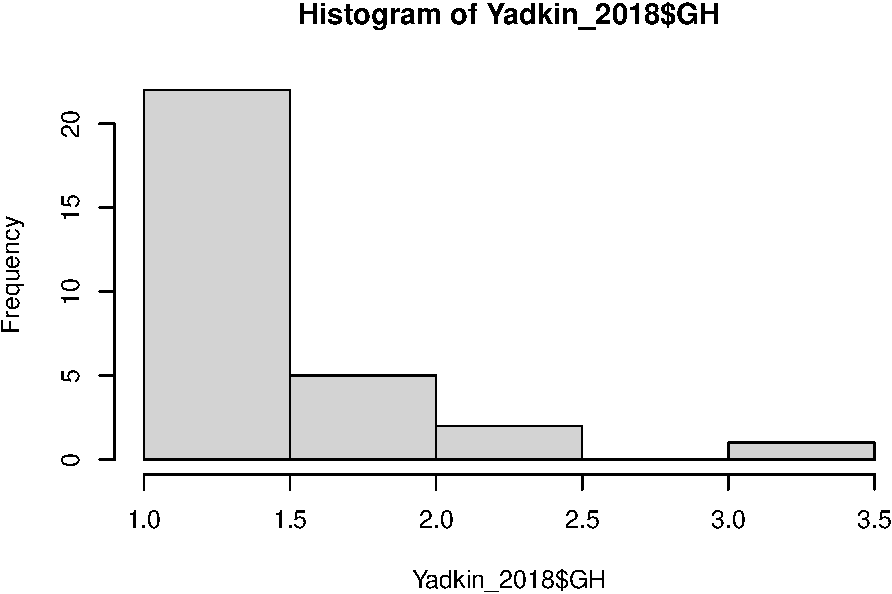
\includegraphics{Project_Template_files/figure-latex/T-Test-1.pdf}

\begin{Shaded}
\begin{Highlighting}[]
\KeywordTok{hist}\NormalTok{(Yadkin_}\DecValTok{2001}\OperatorTok{$}\NormalTok{GH)}
\end{Highlighting}
\end{Shaded}

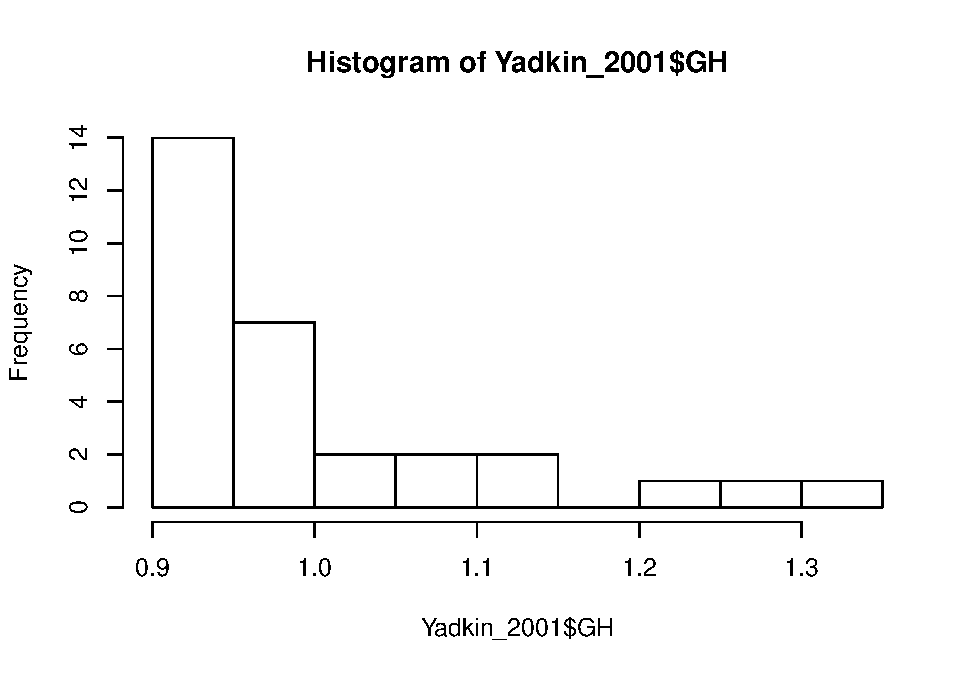
\includegraphics{Project_Template_files/figure-latex/T-Test-2.pdf}

\begin{Shaded}
\begin{Highlighting}[]
\CommentTok{#Run t-test}
\NormalTok{Yadkin_test <-}\StringTok{ }\KeywordTok{t.test}\NormalTok{(Yadkin_}\DecValTok{2001}\OperatorTok{$}\NormalTok{GH, Yadkin_}\DecValTok{2018}\OperatorTok{$}\NormalTok{GH, }\DataTypeTok{var.equal =}\NormalTok{ T)}

\CommentTok{#Graph}
\NormalTok{Yadkin_df <-}\StringTok{ }\KeywordTok{rbind}\NormalTok{(Yadkin_}\DecValTok{2001}\NormalTok{, Yadkin_}\DecValTok{2018}\NormalTok{)}
\KeywordTok{ggplot}\NormalTok{(Yadkin_df, }\KeywordTok{aes}\NormalTok{(}\DataTypeTok{x =} \KeywordTok{factor}\NormalTok{(Year), }\DataTypeTok{y =}\NormalTok{ GH)) }\OperatorTok{+}\StringTok{ }
\StringTok{  }\KeywordTok{geom_boxplot}\NormalTok{() }\OperatorTok{+}\StringTok{ }
\StringTok{  }\KeywordTok{labs}\NormalTok{(}\DataTypeTok{x =} \StringTok{"Year"}\NormalTok{, }\DataTypeTok{y =} \StringTok{"Gage Height (ft)"}\NormalTok{, }\DataTypeTok{title =} \StringTok{"Yadkin 2001 vs. 2018"}\NormalTok{)}
\end{Highlighting}
\end{Shaded}

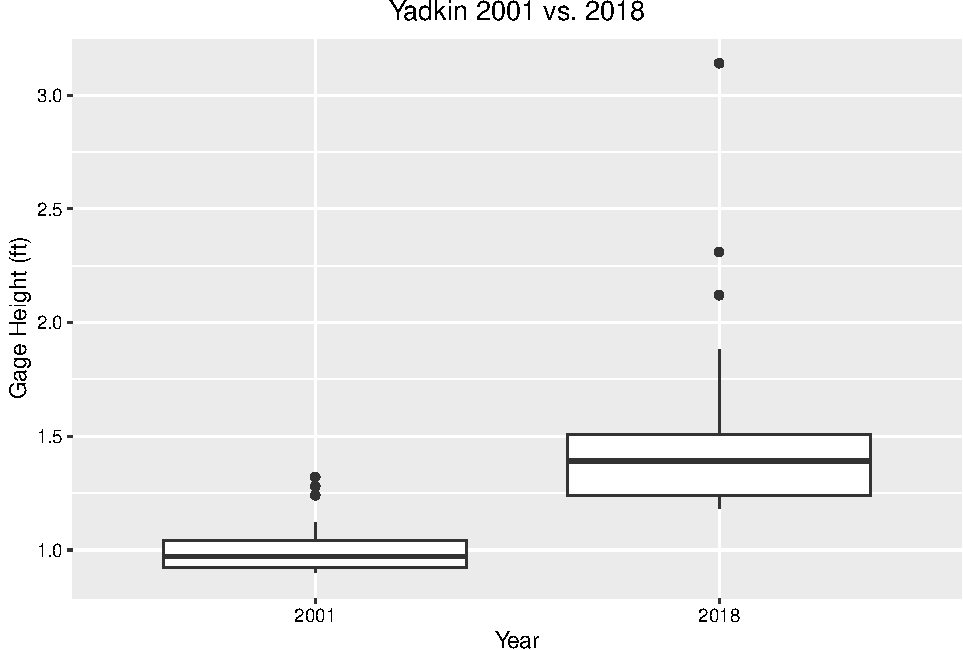
\includegraphics{Project_Template_files/figure-latex/T-Test-3.pdf}

\begin{Shaded}
\begin{Highlighting}[]
\CommentTok{## French Broad - T-Test}
\CommentTok{# Create Dataframes}
\NormalTok{FrenchBroad_}\DecValTok{2001}\NormalTok{ <-}\StringTok{ }\NormalTok{FrenchBroad_sept }\OperatorTok\StringTok{ }\KeywordTok{filter}\NormalTok{(Year}\OperatorTok{==}\StringTok{ }\DecValTok{2001}\NormalTok{)}
\NormalTok{FrenchBroad_}\DecValTok{2018}\NormalTok{ <-}\StringTok{ }\NormalTok{FrenchBroad_sept }\OperatorTok\StringTok{ }\KeywordTok{filter}\NormalTok{(Year}\OperatorTok{==}\StringTok{ }\DecValTok{2018}\NormalTok{)}

\CommentTok{#Check assumptions}
\NormalTok{FrenchBroad_var <-}\StringTok{ }\KeywordTok{var.test}\NormalTok{(FrenchBroad_}\DecValTok{2001}\OperatorTok{$}\NormalTok{GH, FrenchBroad_}\DecValTok{2018}\OperatorTok{$}\NormalTok{GH)}
\KeywordTok{sd}\NormalTok{(FrenchBroad_}\DecValTok{2001}\OperatorTok{$}\NormalTok{GH)}\OperatorTok{/}\KeywordTok{sd}\NormalTok{(FrenchBroad_}\DecValTok{2018}\OperatorTok{$}\NormalTok{GH)}
\end{Highlighting}
\end{Shaded}

\begin{verbatim}
## [1] 0.5959884
\end{verbatim}

\begin{Shaded}
\begin{Highlighting}[]
\KeywordTok{hist}\NormalTok{(FrenchBroad_}\DecValTok{2018}\OperatorTok{$}\NormalTok{GH)}
\end{Highlighting}
\end{Shaded}

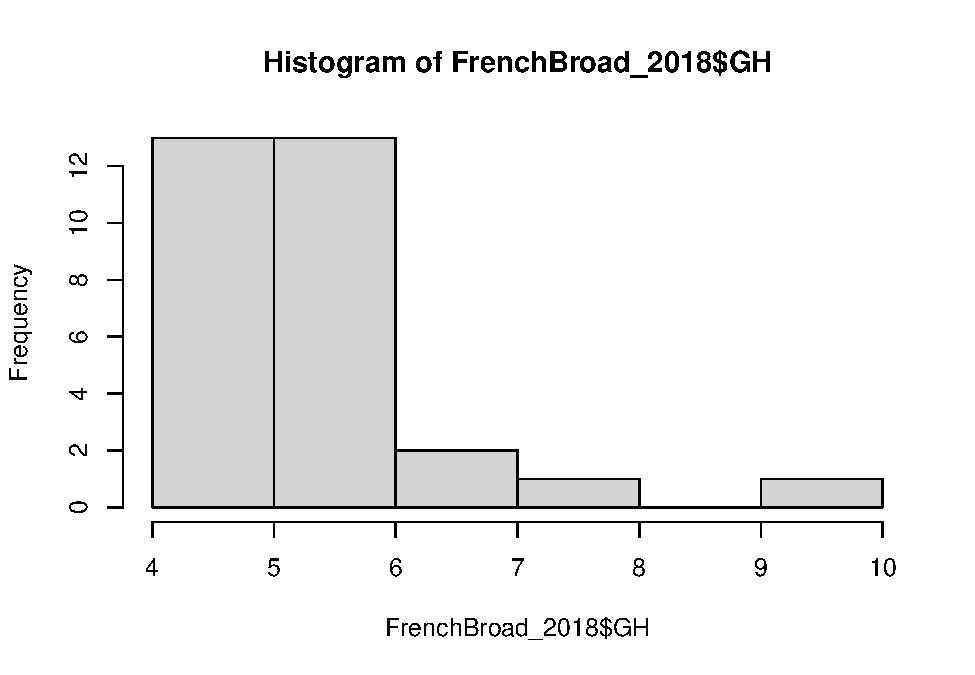
\includegraphics{Project_Template_files/figure-latex/T-Test-4.pdf}

\begin{Shaded}
\begin{Highlighting}[]
\KeywordTok{hist}\NormalTok{(FrenchBroad_}\DecValTok{2001}\OperatorTok{$}\NormalTok{GH)}
\end{Highlighting}
\end{Shaded}

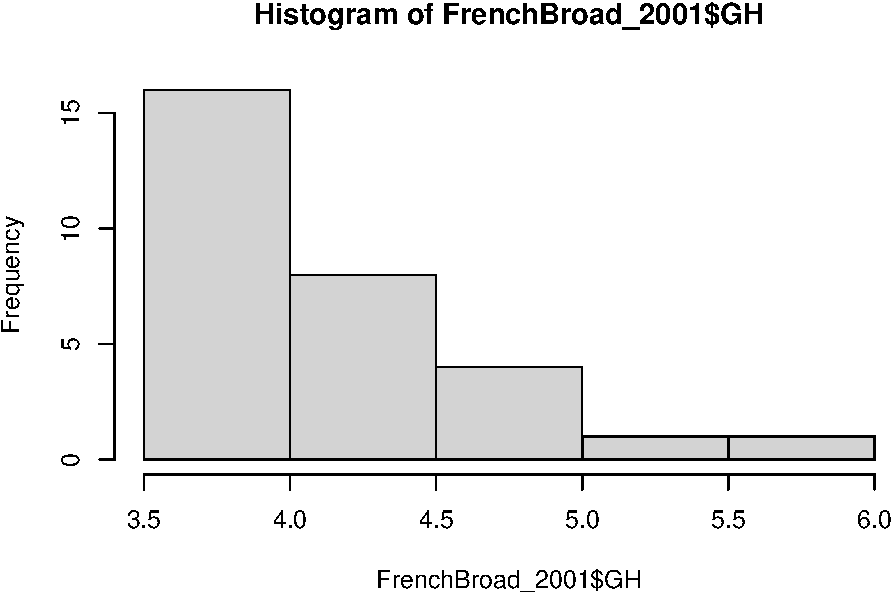
\includegraphics{Project_Template_files/figure-latex/T-Test-5.pdf}

\begin{Shaded}
\begin{Highlighting}[]
\CommentTok{#Run t-test}
\NormalTok{FrenchBroad_test <-}\StringTok{ }\KeywordTok{t.test}\NormalTok{(FrenchBroad_}\DecValTok{2001}\OperatorTok{$}\NormalTok{GH, FrenchBroad_}\DecValTok{2018}\OperatorTok{$}\NormalTok{GH, }\DataTypeTok{var.equal =}\NormalTok{ T)}

\CommentTok{#Graph}
\NormalTok{FrenchBroad_df <-}\StringTok{ }\KeywordTok{rbind}\NormalTok{(FrenchBroad_}\DecValTok{2001}\NormalTok{, FrenchBroad_}\DecValTok{2018}\NormalTok{)}
\KeywordTok{ggplot}\NormalTok{(FrenchBroad_df, }\KeywordTok{aes}\NormalTok{(}\DataTypeTok{x =} \KeywordTok{factor}\NormalTok{(Year), }\DataTypeTok{y =}\NormalTok{ GH)) }\OperatorTok{+}\StringTok{ }
\StringTok{  }\KeywordTok{geom_boxplot}\NormalTok{() }\OperatorTok{+}\StringTok{ }
\StringTok{  }\KeywordTok{labs}\NormalTok{(}\DataTypeTok{x =} \StringTok{"Year"}\NormalTok{, }\DataTypeTok{y =} \StringTok{"Gage Height (ft)"}\NormalTok{, }\DataTypeTok{title =} \StringTok{"French Broad 2001 vs. 2018"}\NormalTok{)}
\end{Highlighting}
\end{Shaded}

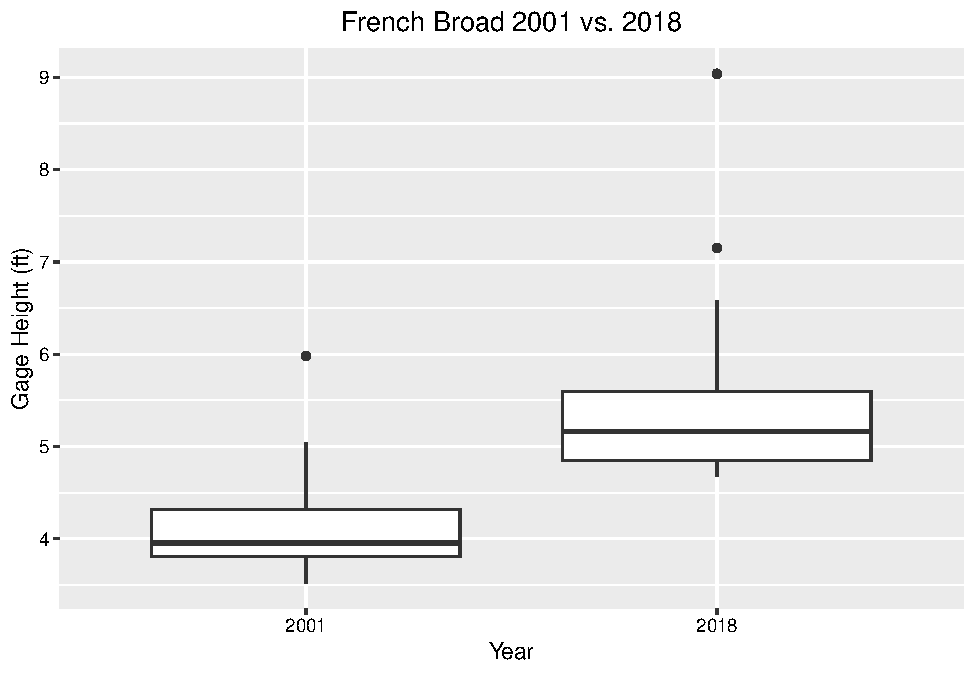
\includegraphics{Project_Template_files/figure-latex/T-Test-6.pdf}

\begin{Shaded}
\begin{Highlighting}[]
\CommentTok{## Mills - T-Test}
\CommentTok{# Create Dataframes}
\NormalTok{Mills_}\DecValTok{2001}\NormalTok{ <-}\StringTok{ }\NormalTok{Mills_sept }\OperatorTok\StringTok{ }\KeywordTok{filter}\NormalTok{(Year}\OperatorTok{==}\StringTok{ }\DecValTok{2001}\NormalTok{)}
\NormalTok{Mills_}\DecValTok{2018}\NormalTok{ <-}\StringTok{ }\NormalTok{Mills_sept }\OperatorTok\StringTok{ }\KeywordTok{filter}\NormalTok{(Year}\OperatorTok{==}\StringTok{ }\DecValTok{2018}\NormalTok{)}

\CommentTok{#Check assumptions}
\NormalTok{Mills_var <-}\StringTok{ }\KeywordTok{var.test}\NormalTok{(Mills_}\DecValTok{2001}\OperatorTok{$}\NormalTok{GH, Mills_}\DecValTok{2018}\OperatorTok{$}\NormalTok{GH)}
\KeywordTok{sd}\NormalTok{(Mills_}\DecValTok{2001}\OperatorTok{$}\NormalTok{GH)}\OperatorTok{/}\KeywordTok{sd}\NormalTok{(Mills_}\DecValTok{2018}\OperatorTok{$}\NormalTok{GH)}
\end{Highlighting}
\end{Shaded}

\begin{verbatim}
## [1] 0.6612318
\end{verbatim}

\begin{Shaded}
\begin{Highlighting}[]
\KeywordTok{hist}\NormalTok{(Mills_}\DecValTok{2018}\OperatorTok{$}\NormalTok{GH)}
\end{Highlighting}
\end{Shaded}

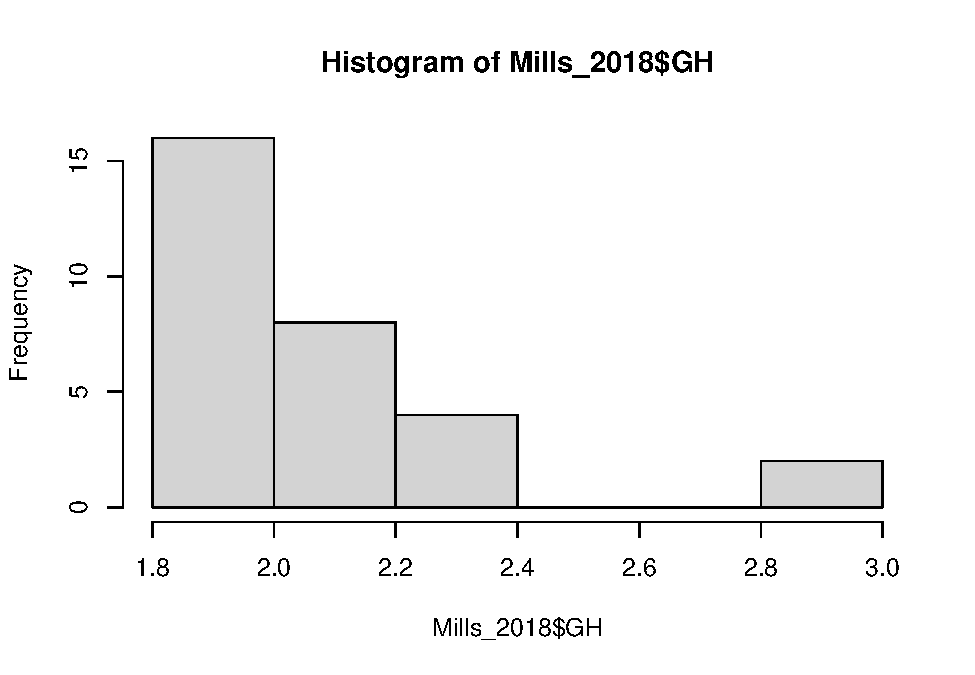
\includegraphics{Project_Template_files/figure-latex/T-Test-7.pdf}

\begin{Shaded}
\begin{Highlighting}[]
\KeywordTok{hist}\NormalTok{(Mills_}\DecValTok{2001}\OperatorTok{$}\NormalTok{GH)}
\end{Highlighting}
\end{Shaded}

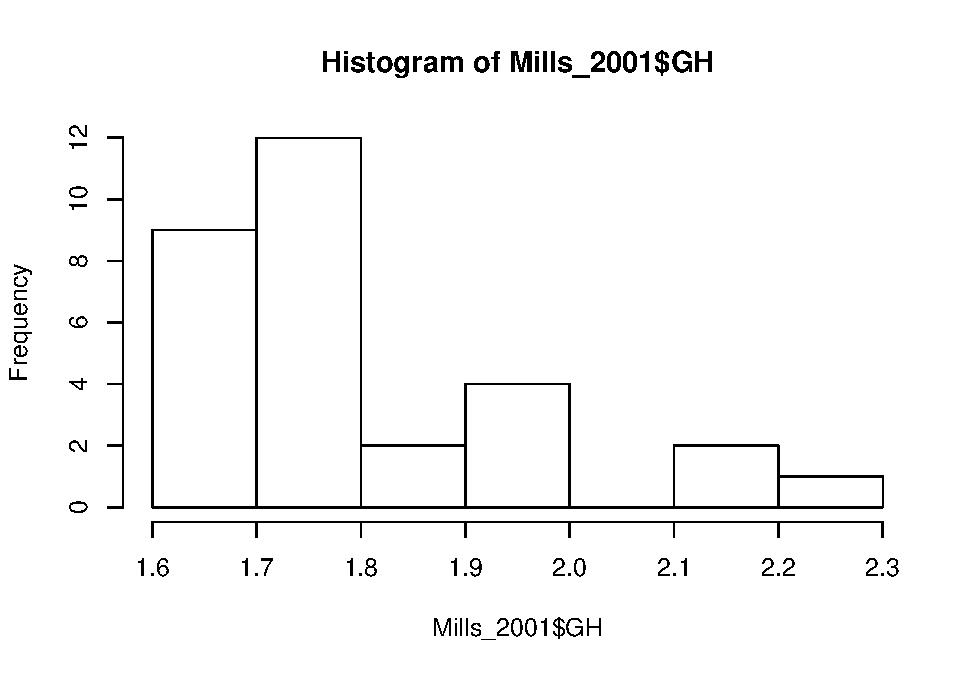
\includegraphics{Project_Template_files/figure-latex/T-Test-8.pdf}

\begin{Shaded}
\begin{Highlighting}[]
\CommentTok{#Run t-test}
\NormalTok{Mills_test <-}\StringTok{ }\KeywordTok{t.test}\NormalTok{(Mills_}\DecValTok{2001}\OperatorTok{$}\NormalTok{GH, Mills_}\DecValTok{2018}\OperatorTok{$}\NormalTok{GH, }\DataTypeTok{var.equal =}\NormalTok{ T)}

\CommentTok{#Graph}
\NormalTok{Mills_df <-}\StringTok{ }\KeywordTok{rbind}\NormalTok{(Mills_}\DecValTok{2001}\NormalTok{, Mills_}\DecValTok{2018}\NormalTok{)}
\KeywordTok{ggplot}\NormalTok{(Mills_df, }\KeywordTok{aes}\NormalTok{(}\DataTypeTok{x =} \KeywordTok{factor}\NormalTok{(Year), }\DataTypeTok{y =}\NormalTok{ GH)) }\OperatorTok{+}\StringTok{ }
\StringTok{  }\KeywordTok{geom_boxplot}\NormalTok{() }\OperatorTok{+}\StringTok{ }
\StringTok{  }\KeywordTok{labs}\NormalTok{(}\DataTypeTok{x =} \StringTok{"Year"}\NormalTok{, }\DataTypeTok{y =} \StringTok{"Gage Height (ft)"}\NormalTok{, }\DataTypeTok{title =} \StringTok{"Mills 2001 vs. 2018"}\NormalTok{)     }
\end{Highlighting}
\end{Shaded}

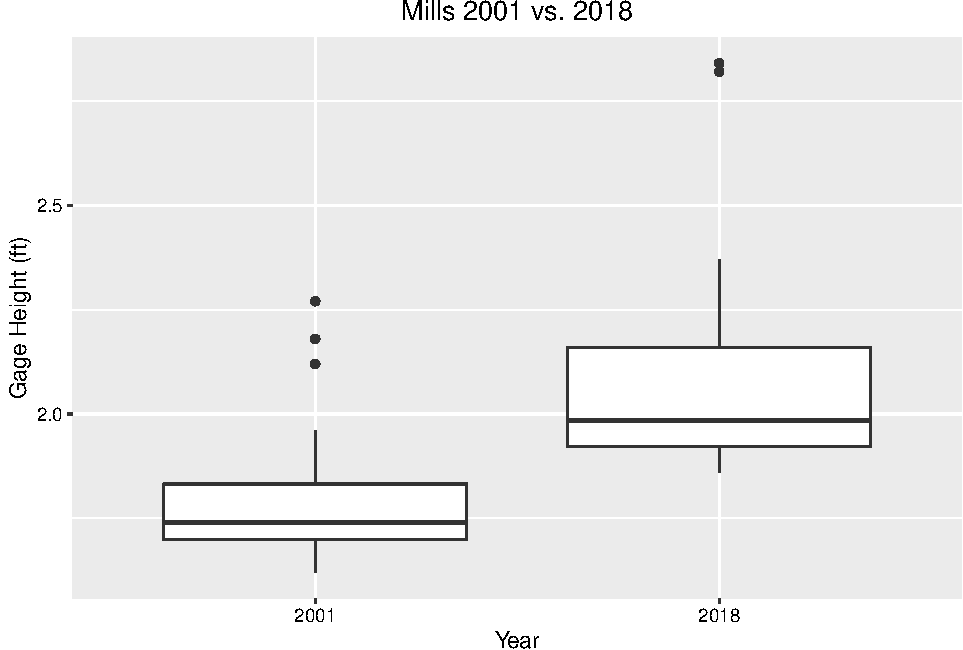
\includegraphics{Project_Template_files/figure-latex/T-Test-9.pdf}

\begin{Shaded}
\begin{Highlighting}[]
\CommentTok{#Create Table of Results}
\NormalTok{Results_df <-}\StringTok{ }\KeywordTok{data.frame}\NormalTok{(}\StringTok{"River_Name"}\NormalTok{ =}\StringTok{ }\KeywordTok{c}\NormalTok{(}\StringTok{'Yadkin River'}\NormalTok{, }\StringTok{'Mills River'}\NormalTok{, }
                                          \StringTok{'French Broad River'}\NormalTok{),}
                 \StringTok{"Average_GH_2001"}\NormalTok{ =}\StringTok{ }\KeywordTok{c}\NormalTok{(}\KeywordTok{mean}\NormalTok{(Yadkin_}\DecValTok{2001}\OperatorTok{$}\NormalTok{GH), }\KeywordTok{mean}\NormalTok{(Mills_}\DecValTok{2001}\OperatorTok{$}\NormalTok{GH),}
                                       \KeywordTok{mean}\NormalTok{(FrenchBroad_}\DecValTok{2001}\OperatorTok{$}\NormalTok{GH)),}
                 \StringTok{"Average_GH_2018"}\NormalTok{ =}\StringTok{ }\KeywordTok{c}\NormalTok{(}\KeywordTok{mean}\NormalTok{(Yadkin_}\DecValTok{2018}\OperatorTok{$}\NormalTok{GH), }\KeywordTok{mean}\NormalTok{(Mills_}\DecValTok{2018}\OperatorTok{$}\NormalTok{GH),}
                                       \KeywordTok{mean}\NormalTok{(FrenchBroad_}\DecValTok{2018}\OperatorTok{$}\NormalTok{GH)),}
                 \StringTok{"var.test_Result"}\NormalTok{ =}\StringTok{ }\KeywordTok{c}\NormalTok{(Yadkin_var}\OperatorTok{$}\NormalTok{statistic, Mills_var}\OperatorTok{$}\NormalTok{statistic,}
\NormalTok{                                       FrenchBroad_var}\OperatorTok{$}\NormalTok{statistic),}
                 \StringTok{"T-Statistic"}\NormalTok{ =}\StringTok{ }\KeywordTok{c}\NormalTok{(Yadkin_test}\OperatorTok{$}\NormalTok{statistic, Mills_test}\OperatorTok{$}\NormalTok{statistic,}
\NormalTok{                                       FrenchBroad_test}\OperatorTok{$}\NormalTok{statistic),}
                 \StringTok{"P-Value"}\NormalTok{ =}\StringTok{ }\KeywordTok{c}\NormalTok{(Yadkin_test}\OperatorTok{$}\NormalTok{p.value, Mills_test}\OperatorTok{$}\NormalTok{p.value,}
\NormalTok{                               FrenchBroad_test}\OperatorTok{$}\NormalTok{p.value))}

\KeywordTok{kable}\NormalTok{(Results_df, }\DataTypeTok{col.names =} \KeywordTok{c}\NormalTok{(}\StringTok{"River Name"}\NormalTok{, }\StringTok{"2001 Average GH"}\NormalTok{, }
                                \StringTok{"2018 Average GH"}\NormalTok{, }\StringTok{"var.test Result"}\NormalTok{, }
                                \StringTok{"T-Statistic"}\NormalTok{, }\StringTok{"P-Value"}\NormalTok{), }
                  \DataTypeTok{caption =} \StringTok{"Results"}\NormalTok{, }\DataTypeTok{digits =} \KeywordTok{c}\NormalTok{(}\DecValTok{0}\NormalTok{, }\DecValTok{2}\NormalTok{, }\DecValTok{2}\NormalTok{, }\DecValTok{2}\NormalTok{, }\DecValTok{2}\NormalTok{, }\DecValTok{8}\NormalTok{)) }\OperatorTok\StringTok{ }
\StringTok{  }\KeywordTok{column_spec}\NormalTok{(}\DecValTok{1}\OperatorTok{:}\DecValTok{5}\NormalTok{,}\DataTypeTok{border_left =}\NormalTok{ T, }\DataTypeTok{border_right =}\NormalTok{ T) }\OperatorTok
\StringTok{  }\KeywordTok{kable_styling}\NormalTok{()}
\end{Highlighting}
\end{Shaded}

\begin{table}

\caption{\label{tab:T-Test}Results}
\centering
\begin{tabular}[t]{|>{}l|||>{}r|||>{}r|||>{}r|||>{}r||r}
\hline
River Name & 2001 Average GH & 2018 Average GH & var.test Result & T-Statistic & P-Value\\
\hline
Yadkin River & 1.00 & 1.49 & 0.07 & -6.22 & 6.00e-08\\
\hline
Mills River & 1.80 & 2.08 & 0.44 & -5.37 & 1.46e-06\\
\hline
French Broad River & 4.12 & 5.41 & 0.36 & -6.72 & 1.00e-08\\
\hline
\end{tabular}
\end{table}

\hypertarget{question-1-has-gage-height-changed-over-2000-2020-for-september-from-hurricanes}{%
\subsection{Question 1: Has gage height changed over 2000-2020 for
September from
hurricanes?}\label{question-1-has-gage-height-changed-over-2000-2020-for-september-from-hurricanes}}

Yadkin River, Mills River, and French Broad River had a significant
(p-value \textless{} 0.05) monotonic upward trend. French Broad River
had the largest upward trend ( ) and Yadkin River and Mills River had
the smallest upward trend (0.0218).

\hypertarget{question-2-how-much-does-a-stream-gage-height-change-after-a-hurricane}{%
\subsection{Question 2: How much does a stream gage height change after
a
hurricane?}\label{question-2-how-much-does-a-stream-gage-height-change-after-a-hurricane}}

Yadkin River Mills River French Broad River

\hypertarget{question-3-are-gage-heights-significantly-different-between-2001-and-2018}{%
\subsection{Question 3: Are gage heights significantly different between
2001 and
2018?}\label{question-3-are-gage-heights-significantly-different-between-2001-and-2018}}

The mean gage heights for each river was higher in 2018 than in 2001,
and these differences were statistically significant. Since the
t-statistic for the Yadkin, Mills, and French Broad Rivers (-6.22,
-5.37, and -6.72) are negative, this indicates that the 2018 gage
heights are greater than the 2001 heights. The Yadkin River gage was
0.49 feet higher in 2018 (p-value \textless{} 0.05). The Mills River
gage was 0.28 feet higher in 2018 (p-value \textless{} 0.05). The French
Broad River gage was 1.28 feet higher in 2018 (p-value \textless{}
0.05). A necessary assumption for statistical t-tests is that variances
are approximately equal, with the ratio of variances produced using the
var.test function at around 0.5. It is important to note that this was
not the case for all three rivers studied. Yadkin River was especially
low (0.07) and French Broad River was 0.36. The ratio for Mills River
was appropriate (0.44). Another necessary assumption is that the data
are normally distributed, which was again not the case for all three
rivers in both years. All samples were notably right-skewed; however,
this makes sense given that gage heights are expected to remain around
the same level. The high values that are skewing the distribution of the
data could reflect the increases in gage height due to hurricanes
(especially in 2018) or other unusual events (for example, human
regulation of river flow).\\
With these results, we reject the null hypothesis and conclude that the
average gage heights for 2001 and 2018 are different and that this
difference is statistically significant for all three rivers.

\newpage

\hypertarget{summary-and-conclusions}{%
\section{Summary and Conclusions}\label{summary-and-conclusions}}

Water level has been increasing for the month of September over the last
20 years, based on the significant upward trend from the time series
analysis. Based on National Climatic Data Center Event Report for
Hurricanes, in 2018, 46 people died due to hurricane Florence and
Michael, the only 2 hurricanes to hit that year and in 2016, 28 people
died due to hurricane Matthew. From 2000 - 2012, 41 people in total died
due to hurricanes. Death from hurricanes are usually linked to flooding,
which can cause expose individuals to sewage water, damage
infrastructure making roads and homes dangerous, and potentially drown
victims (Choudhary et al., 2012). Though storms appeared to have
decreased in frequency (there were 48 storms from 2000 - 2010, but only
18 storms from 2011 -- 2020) it is evident that the severity of the
storms has increased, based on both deaths and increasing water levels.
Further research should be done to quantify how much additional water is
deposited per storm and what updates to infrastructure should be done to
account for this additional water. To evaluate increase in hurricane
intensity due to climate change, we compared gage heights between 2001,
a year with no September hurricanes impacting North Carolina, and 2018,
a year with the major Hurricane Florence. The results of our t-test
showed that there was a significant difference in gage height,
indicating that hurricane intensity and flood potential increased. While
it is possible that other factors contributed to this increase in gage
height, our conclusions are supported by existing research studies that
link climate change to increases in hurricane intensity (Emanuel, 1987).

\newpage

\hypertarget{references}{%
\section{References}\label{references}}

Ameli, A. A., \& Creed, I. F. (2019). Does Wetland Location Matter When
Managing Wetlands for Watershed-Scale Flood and Drought Resilience?
Journal of the American Water Resources Association, 55(3), 529--542.
\url{https://doi.org/10.1111/1752-1688.12737}

Carle, M. V. (2011). Estimating wetland losses and gains in coastal
north carolina: 1994-2001. Wetlands, 31(6), 1275--1285.
\url{https://doi.org/10.1007/s13157-011-0242-z}

Choudhary, E., Zane, D. F., Beasley, C., Jones, R., Rey, A., Noe, R. S.,
Martin, C., Wolkin, A. F., \& Bayleyegn, T. M. (2012). Evaluation of
active mortality surveillance system data for monitoring
hurricane-related deaths-texas, 2008. Prehospital and Disaster Medicine,
27(4), 392--397. \url{https://doi.org/10.1017/S1049023X12000957}

Elsner, J. B. (2006). Evidence in support of the climate change-Atlantic
hurricane hypothesis. Geophysical Research Letters, 33(16), 1--3.
\url{https://doi.org/10.1029/2006GL026869}

Emanuel, K. A. (1987). The dependence of hurricane intensity on climate.
Nature, 326, 483--485. \url{https://doi.org/10.1038/326483a0}

James M. Shultz, Ph.D., Duane E. Sands, M.D., James P. Kossin, Ph.D.,
and Sandro Galea, M.D., Dr.~P. H. (2020). Double Environmental Injustice
- Climate Change, Hurricane Dorian, and the Bahamas. The New England
Journal of Medicine, 1--3.

Marsooli, R., \& Lin, N. (2020). Impacts of climate change on hurricane
flood hazards in Jamaica Bay, New York. Climatic Change, 163(4),
2153--2171. \url{https://doi.org/10.1007/s10584-020-02932-x}

Villa, Clifford, et al.~Environmental Justice: Law, Policy \&
Regulation. Carolina Academic Press, 2020.

Violin, C. R., Cada, P., Sudduth, E. B., Hassett, B. A., Penrose, D. L.,
\& Bernhardt, E. S. (2011). Effects of urbanization and urban stream
restoration on the physical and biological structure of stream
ecosystems. Ecological Applications, 21(6), 1932--1949.
\url{https://doi.org/10.1890/10-1551.1}


\end{document}
